\section{线性松弛与原解恢复}
\label{sec:opt-lp-relaxation}

第~\ref{sec:opt-lp-modeling}节看到，产品只能整件生产时，连续模型的解$(4/3,4/3)$不能直接使用。许多离散问题都有类似的结构：候选是有限个点，目标是线性函数。上一节在同一个连续模型内改变数据；本节改变的是问题本身，研究怎样把离散候选放进一个连续的多面体中求解，以及连续解和连续最优值能为原离散问题提供什么。答案分两种情形：若多面体恰好是候选的凸包，最优值不变；若只能用一个更大的多面体，得到的是一个界，原问题的候选还需要另行恢复。

\subsection{精确凸包与线性值保持}
\label{sec:opt-lp-convex-hull}

\paragraph{线性目标在凸包上不变}
设$S\subseteq\mathbb R^d$是非空有限集，目标是线性函数$\bm c^\top\bm x$。凸包$\operatorname{conv}(S)$由$S$中点的全部凸组合组成（见第~\ref{chap:optimization}章），它比$S$大得多，却不会给线性目标带来更好的值。

\begin{theorem}[凸包上的线性值保持]
\label{thm:opt-lp-hull-value}
设$S$是非空有限集。则
\[
  \max_{\bm x\in\operatorname{conv}(S)}\bm c^\top\bm x=\max_{\bm s\in S}\bm c^\top\bm s,
\]
并且$\operatorname{conv}(S)$上的最优解集恰好是$S$中全部最优点的凸包。最小化同理。
\end{theorem}

\begin{proof}
记$M=\max_{\bm s\in S}\bm c^\top\bm s$，有限集上的最大值一定取到。任取$\bm x=\sum_i\lambda_i\bm s_i\in\operatorname{conv}(S)$，$\lambda_i\ge0$，$\sum_i\lambda_i=1$。由线性，
\[
  \bm c^\top\bm x=\sum_i\lambda_i\,\bm c^\top\bm s_i\le\sum_i\lambda_iM=M,
\]
即凸包中任一点的目标值是候选值的加权平均，不超过最大的候选值；而$S\subseteq\operatorname{conv}(S)$，所以两个最大值相等。等号成立当且仅当每个$\lambda_i>0$的$\bm s_i$都满足$\bm c^\top\bm s_i=M$，即$\bm x$只由最优候选组合而成，这给出最优解集的刻画。
\end{proof}

这是线性目标与精确凸包共同给出的结论，两个条件缺一不可。若把目标换成非线性函数，凸组合的目标值不再是加权平均，例如在$S=\{0,1\}$上最大化$x(1-x)$，两个候选的值都是$0$，凸包$[0,1]$上的最大值却在$x=1/2$处取得$1/4$，答案改变了。若把凸包换成一个更大的多面体，最优值一般也会改变，这是下一小节的主题。

\paragraph{最优值保持，输出却可能是分数}
最优值相同，并不意味着在凸包上求解就得到了原问题的解。图~\ref{fig:opt-lp-exact-hull}中$S=\{(0,0),(1,0),(0,1)\}$，在凸包（三角形）上最大化$x_1+x_2$，最优值$1$与原问题相同，但最优面是整条斜边，其中的$(1/2,1/2)$同样最优，却不是原候选。所以“求连续最优值”和“恢复一个原候选”是两个步骤。

\begin{figure}[!htbp]
  \centering
  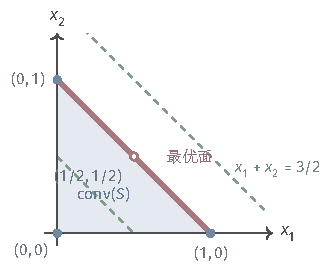
\includegraphics[width=56.257mm]{figures/03-optimization-evolution-and-signals/01-optimization/tikz/c2-exact-hull/figure.pdf}
  \caption{精确凸包上的线性目标。蓝点为三个候选，浅蓝三角形是它们的凸包。最大化$x_1+x_2$的最优值为$1$，与原候选上的最优值相同；红色粗线是最优面，空心点$(1/2,1/2)$在其上，同样最优却不是候选。绿色虚线是值为$1/2$与$3/2$的等值线。}
  \label{fig:opt-lp-exact-hull}
\end{figure}

恢复候选有一条现成的途径。凸包$\operatorname{conv}(S)$的极点都属于$S$：凸包中不属于$S$的点是至少两个不同候选的、系数为正的凸组合，不是极点。若凸包能用有限个线性不等式写出来，单纯形法返回的是基本可行解，即极点（定理~\ref{thm:opt-lp-bfs-extreme}），它自动属于$S$。困难在于前提：对一般的离散问题，凸包的不等式描述可能极为复杂，甚至条数随规模指数增长，无法写出。

网络流是前提成立的重要特例。在第~\ref{sec:opt-lp-reduced-cost}小节对照过的最小费用流中，供需量和容量都是整数时，网络单纯形法的基本可行解在生成树上逐个叶子用守恒式求出，每一步只做整数的加减，所以每个基本可行解都是整数流。线性规划在这里自动给出整数解，依靠的是关联矩阵的特殊结构；一般线性规划没有这一性质，不能期待它的顶点是整数点。

\subsection{外逼近松弛与原解恢复}
\label{sec:opt-lp-outer}

\paragraph{用更大的多面体换取可解性}
写不出精确凸包时，常用的做法是保留原问题中的线性约束，只把“变量取整数”放宽为“变量在区间中”。这样得到的多面体$R$包含全部原候选，但一般比凸包大，称为原问题的\term{线性规划松弛}（linear programming relaxation），也是对凸包的一种\term{外逼近}（outer approximation）。由$S\subseteq R$立即得到：对最大化问题，$\max_R\bm c^\top\bm x\ge\max_S\bm c^\top\bm x$，松弛值是原最优值的上界；对最小化问题，松弛值是下界。

\begin{example}[二元选择]
\label{ex:opt-lp-binary-relaxation}
考虑
\[
  \max\ x_1+x_2\quad\text{s.t.}\quad 2x_1+2x_2\le3,\quad x_1,x_2\in\{0,1\}.
\]
可行候选是$(0,0)$、$(1,0)$、$(0,1)$，$(1,1)$违反约束，所以整数最优值为$1$。把$x_i\in\{0,1\}$放宽为$0\le x_i\le1$，得到图~\ref{fig:opt-lp-outer-relaxation}(a)中的五边形，最优值为$3/2$，在线段$x_1+x_2=3/2$（$1/2\le x_1\le1$）上取得，例如$(3/4,3/4)$与$(1,1/2)$。精确凸包是三角形$x_1+x_2\le1$，五边形比它多出一块。松弛值与原最优值之差$3/2-1=1/2$称为这个实例的加性\term{整数间隙}（integrality gap）；它衡量的是松弛的界偏离了多少，而不是某个算法的误差。
\end{example}

\begin{figure}[!htbp]
  \centering
  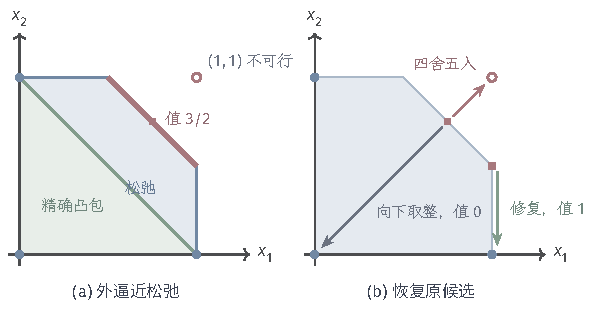
\includegraphics[width=100.986mm]{figures/03-optimization-evolution-and-signals/01-optimization/tikz/c2-outer-relaxation/figure.pdf}
  \caption{二元选择问题的线性规划松弛与候选恢复。(a) 浅蓝五边形是松弛$\{0\le x_i\le1,\ x_1+x_2\le3/2\}$，浅绿三角形是精确凸包；蓝点是可行候选，红圈$(1,1)$违反约束。红色粗线是松弛的最优面，值为$3/2$，红方块$(3/4,3/4)$是其中一点。(b) 三种恢复方式：从$(3/4,3/4)$四舍五入得到不可行的$(1,1)$；向下取整得到可行但值为$0$的$(0,0)$；从$(1,1/2)$把分数坐标降为$0$，得到值为$1$的可行候选$(1,0)$。}
  \label{fig:opt-lp-outer-relaxation}
\end{figure}

\paragraph{从松弛解恢复候选}
松弛给出的点通常不是原候选，需要一个恢复步骤，而恢复后的点要分别检查可行性和目标损失。图~\ref{fig:opt-lp-outer-relaxation}(b)比较了三种做法。若求解器返回$(3/4,3/4)$，四舍五入得到$(1,1)$，违反容量约束；向下取整得到$(0,0)$，可行但获利为$0$，损失了全部收益。若求解器返回顶点$(1,1/2)$，只把唯一的分数坐标降为零，得到$(1,0)$，它满足原约束，获利为$1$。可见恢复规则必须依据原约束设计：对这类“容量不超过”的约束，把变量往下调总能保持可行，但损失多少取决于从哪个松弛解出发、怎样调整。

\paragraph{区间证书}
恢复得到的可行候选与松弛值一起，构成原最优值的一个区间。对最大化问题，可行候选的值是下界，松弛值是上界：二元选择中原最优值落在$[1,3/2]$中。若目标在候选上只取整数，上界还可以向下取整：最优值不超过$\lfloor3/2\rfloor=1$，而$(1,0)$达到$1$，这就证明了$(1,0)$最优。回到章首的作坊：连续松弛值$20/3$说明整件生产的获利不超过$\lfloor20/3\rfloor=6$，而$(2,0)$获利$6$，所以它是整数最优解；把$(4/3,4/3)$向下取整得到的$(1,1)$只获利$5$。

\paragraph{能承诺什么，不能承诺什么}
线性规划松弛是连续问题，可以用单纯形法或第~\ref{chap:constrained-optimization}章的内点法求解，但这并不使离散原问题变得容易：一般的整数线性规划仍是困难问题，松弛只提供一个界和一个恢复的起点。整数间隙可能很大，此时区间证书很宽，恢复出的候选也可能很差；收紧松弛需要加入更多有效不等式，或采用更强的松弛。把变量提升为矩阵、以半正定约束代替线性约束的半正定松弛，留到第~\ref{chap:constrained-optimization}章讨论。
